%% Direttive TeXworks:
% !TeX root = ../report.tex
% !TEX encoding = UTF-8 Unicode
% !TeX spellcheck = it-IT

\subsection{Sprint Planning}\labelssec{sp2:planning}

Durante lo Sprint precedente descritto nella \Cref{sec:sprint1}, è stato realizzato un sistema locale di massima, che implementasse i requisiti principali del sistema richiesto.
Come detto nella \Cref{ssec:sp1:review}, durante la fase di \nameref{ssec:sp1:review} non ci sono state richieste aggiuntive da parte del committente, né correzioni su quanto prodotto, di conseguenza si può procedere evolvendo il sistema.

Alla fine di questo Sprint si vuole avere un sistema che realizzi le funzionalità principali della fase di esplorazione:
in particolare, è importante avere un robot che possa muoversi all'interno di uno spazio e generare una mappa dello spazio esplorato.

Non è ancora ritenuto necessario che il robot di test sia fisico, ma deve esserne mantenuto il supporto per sviluppi negli Sprint futuri.

\subsection{Analisi dei requisiti}\labelssec{sp2:req_analysis}

Dopo aver delineato l'obiettivo di massima durante la fase di \nameref{ssec:sp2:planning}, si è individuato i requisiti specifici da realizzare durante questo Sprint:

\begin{description}
  \item[\requirementref{R-explore}]
    a differenza dello \nameref{sec:sprint1}, questa volta durante la fase di esplorazione il robot dovrà realmente muoversi all'interno di un dato spazio.
    I problemi principali di questa fase riguardano come gestire il movimento a livello logico (ad esempio, suddividendo la mappa in celle) e fisico (per esempio, utilizzando un modello a tempo);
    inoltre, è anche da considerare la logica con la quale lo spazio viene esplorato e successivamente memorizzato.

  \item[\requirementref{R-stopAtBag}]
    il robot non deve schiantarsi durante la fase di esplorazione;
    deve dunque potersi fermare se incontra un ostacolo (che si assume da requisiti essere fisso).

  \item[\requirementref{R-backHome}]
    il robot deve poter tornare alla base una volta terminata la fase di esplorazione.
\end{description}

Devo ovviamente essere mantenuti soddisfatti i requisiti già implementati.

\subsection{Analisi del problema}\labelssec{sp2:prob_analysis}

A seguito dell'analisi dei requisiti, sono state fatte diverse considerazioni sui problemi emersi;
di seguito si descrive nel dettaglio ciascuna di queste.

\subsubsection{Celle come unità di movimento}\labelsssec{sp2:cells}

Un problema sorto durante la progettazione è stato il modo nel quale il robot esplora ed è consapevole della sua posizione nello spazio.
Per risolvere questo problema e per permettere la costruzione di una mappa in modo semplice, si è ritenuto che la cosa migliore da fare fosse suddividere lo spazio in celle grandi quanto il robot stesso.

In questo modo, il robot può navigare lo spazio muovendosi di cella in cella, come se fossero le pedine di una scacchiera.

\subsubsection{Planner}\labelsssec{sp2:planner}

Per rispettare il requisito \requirementref{R-explore}, il problema della logica di esplorazione della hall risulta abbastanza complesso da affrontare e risolvere in modo ottimale con le conoscenze attualmente possedute.
Sarebbe invece ottimale avere un componente che organizzi le mosse del robot in modo da consentire un'esplorazione ``intelligente''.

In questo caso è tornato utile il software già presente nella software house che ha permesso di ottenere una sequenza di mosse da eseguire fornendogli una destinazione obiettivo.
Oltre a gestire la pianificazione delle azioni questo mantiene internamente una mappa dell'ambiente che stiamo esplorando.

Questo modulo fa uso di una libreria esterna sviluppata dalla \textit{Computer Science Division} della UC Berkeley, AIMA\footnote{\url{https://github.com/aimacode/aima-java}}.
Essa fornisce un'implementazione dell'algoritmo di AI descritto nel libro \textit{Artificial Intelligence --- A Modern Approach 3rd Edition}~\cite{Russell:2009:AIM:1671238}, che permette di ottenere le azioni da eseguire per ottenere un goal.

Nel modulo è già presente un modello di mappa interamente realizzato in Java, utilizzato per individuare i percorsi da intraprendere durante l'esplorazione.

\subsubsection{Movimento atomico}\labelsssec{sp2:atomic}

L'impiego del planner fornito dalla sfotware house impone una modalità di gestione dello spazio ben specifica:
come detto nella \Cref{sssec:sp2:planner}, la mappa è costituita da celle e il planner fornisce l'indicazione dei movimenti da cella a cella.
È dunque compito del robot sapere come muoversi da una cella all'altra atomicamente.

Dato che il \texttt{robot\_adapter} realizzato è in grado di eseguire solo comandi grezzi, si è deciso di aggiungere un nuovo componente: \texttt{robot\_advanced}.
Nella propria versione ``avanzata'', il robot è in grado di svolgere movimenti atomici utilizzando il \texttt{robot\_adapter} come livello inferiore, andando a definire un livello di astrazione superiore.

Data l'impossibilità di dotare il robot di ulteriori sensori, l'unica \textit{unità di misura} per gestire i movimenti atomici possibile è il \textbf{tempo}:
il robot si muove contando il tempo trascorso ed è consapevole del tempo necessario per spostarsi dalla cella corrente alla successiva.

L'introduzione di questo livello di astrazione aggiuntivo ha permesso alla \texttt{robot\_mind} di occuparsi esclusivamente della gestione del piano, sfruttando il \textit{planner} per calcolare il percorso e incaricando il robot di eseguire le singole azioni.

\subsubsection{One cell forward}\labelsssec{sp2:ocf}

A differenza dei movimenti rotatori, che vanno semplicemente eseguiti, lo spostamento in avanti può causare lo scontro con un ostacolo;
in tal caso, il robot deve essere in grado di riposizionarsi nella cella dalla quale era partito, senza lasciarlo in uno stato inconsistente.

Questa operazione è più complessa e, poiché la software house metteva già a disposizione un componente che si occupa di tale operazione, si è deciso di riutilizzarlo nel sistema:
questo componente è il \texttt{One cell forward}.

È importante specificare che il sonar fisico sarebbe in grado di restituire la distanza dell'ostacolo che ha di fronte
(con una precisione molto variabile a seconda della qualità del sensore e della tipologia di superfici con cui sono fatti i muri),
perciò potrebbe fermarsi ancora prima di partire;
il robot virtuale è invece in grado di rilevare l'ostacolo solo dopo essercisi scontrato.

Per questa particolare scelta, l'approccio \textit{bottom-up} utilizzato nasce anche dalla presenza di strumenti, all'interno della software house, che potessero gestire la problematica perfino in un sistema complesso.

\subsection{Architettura logica in output all'analisi del problema}\labelssec{sp2:arch_logica_prob}

Continuando con un approccio top-down, le nuove entità e i loro comportamenti sono rappresentati dagli schemi seguenti:

\begin{figure}[H]
  \centering
  % \includegv[width=\textwidth]{res/sprint2/onecellforward}
  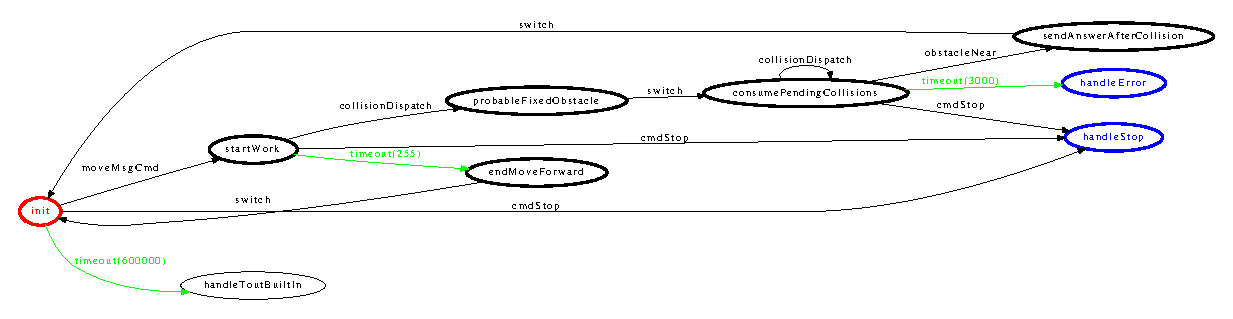
\includegraphics[width=\textwidth]{res/sprint2/onecellforward}
  \caption{One Cell Forward}%
  \label{fig:sp2:ocf}
\end{figure}

\begin{figure}[H]
  \centering
  % \includegv[width=\textwidth]{res/sprint2/robot_adapter}
  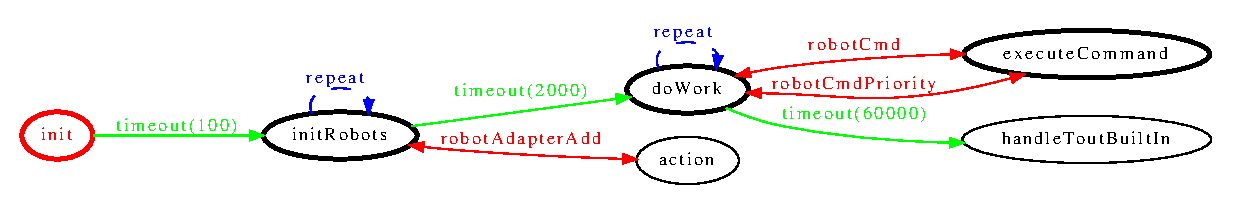
\includegraphics[width=\textwidth]{res/sprint2/robot_adapter}
  \caption{Robot Adapter}%
  \label{fig:sp2:r_adpt}
\end{figure}

\begin{figure}[H]
  \centering
  % \includegv[width=\textwidth]{res/sprint2/robot_advanced}
  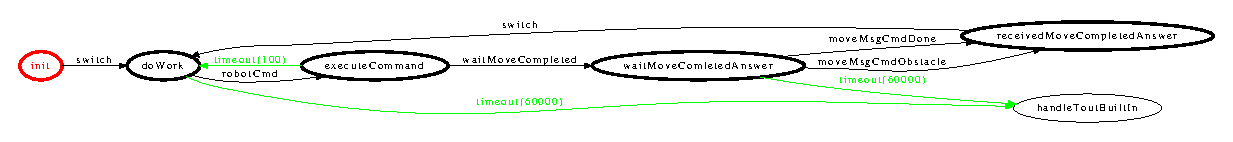
\includegraphics[width=\textwidth]{res/sprint2/robot_advanced}
  \caption{Robot Advanced}%
  \label{fig:sp2:r_adv}
\end{figure}

% \begin{figure}[H]
%   \centering
%   % \includegv[width=\textwidth]{res/sprint2/robot_discovery_mind}
%   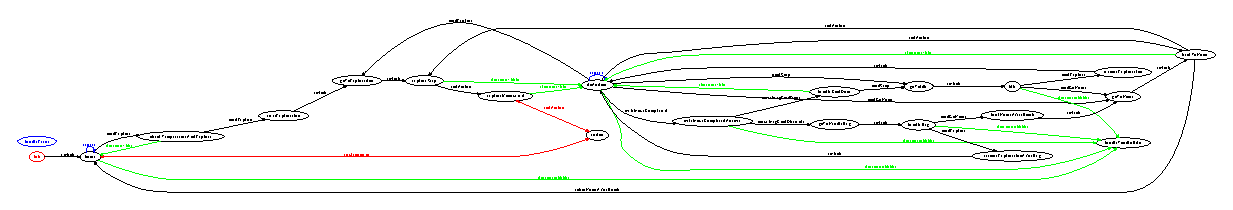
\includegraphics[width=\textwidth]{res/sprint2/robot_discovery_mind}
%   \caption{Mind del Robot Discovery}%
%   \label{fig:sp2:rdm}
% \end{figure}

% \begin{figure}[H]
%   \centering
%   % \includegv[width=\textwidth]{res/sprint2/robot_retriever_mind}
%   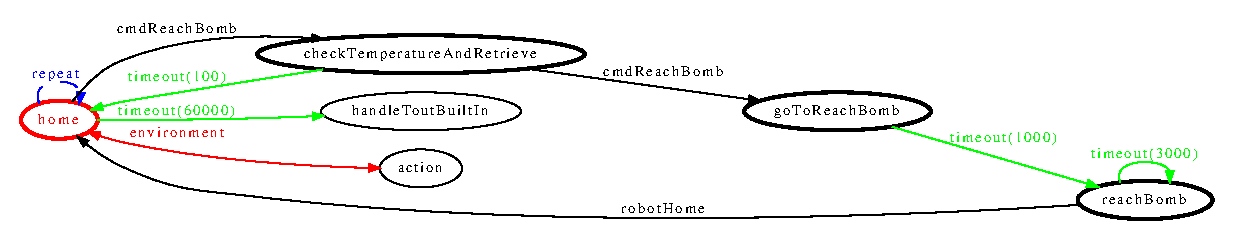
\includegraphics[width=\textwidth]{res/sprint2/robot_retriever_mind}
%   \caption{Mind del Robot Retriever}%
%   \label{fig:sp2:rrm}
% \end{figure}

% \begin{figure}[H]
%   \centering
%   % \includegv[width=0.5\textwidth]{res/sprint2/world_observer}
%   \includegraphics[width=0.5\textwidth]{res/sprint2/world_observer}
%   \caption{World Observer}%
%   \label{fig:sp2:wo}
% \end{figure}

A livello di interazioni, come detto nelle \nameCrefs{ssec:sp2:arch_logica_prob} precedenti, il sistema mantiene le interazioni precedenti ed aggiunge quelle relative all'esplorazione;
di conseguenza, di seguito in \Cref{fig:sp2:explore} si rappresenta l'interazione tra gli attori coinvolti:

\begin{figure}[H]
  \centering
  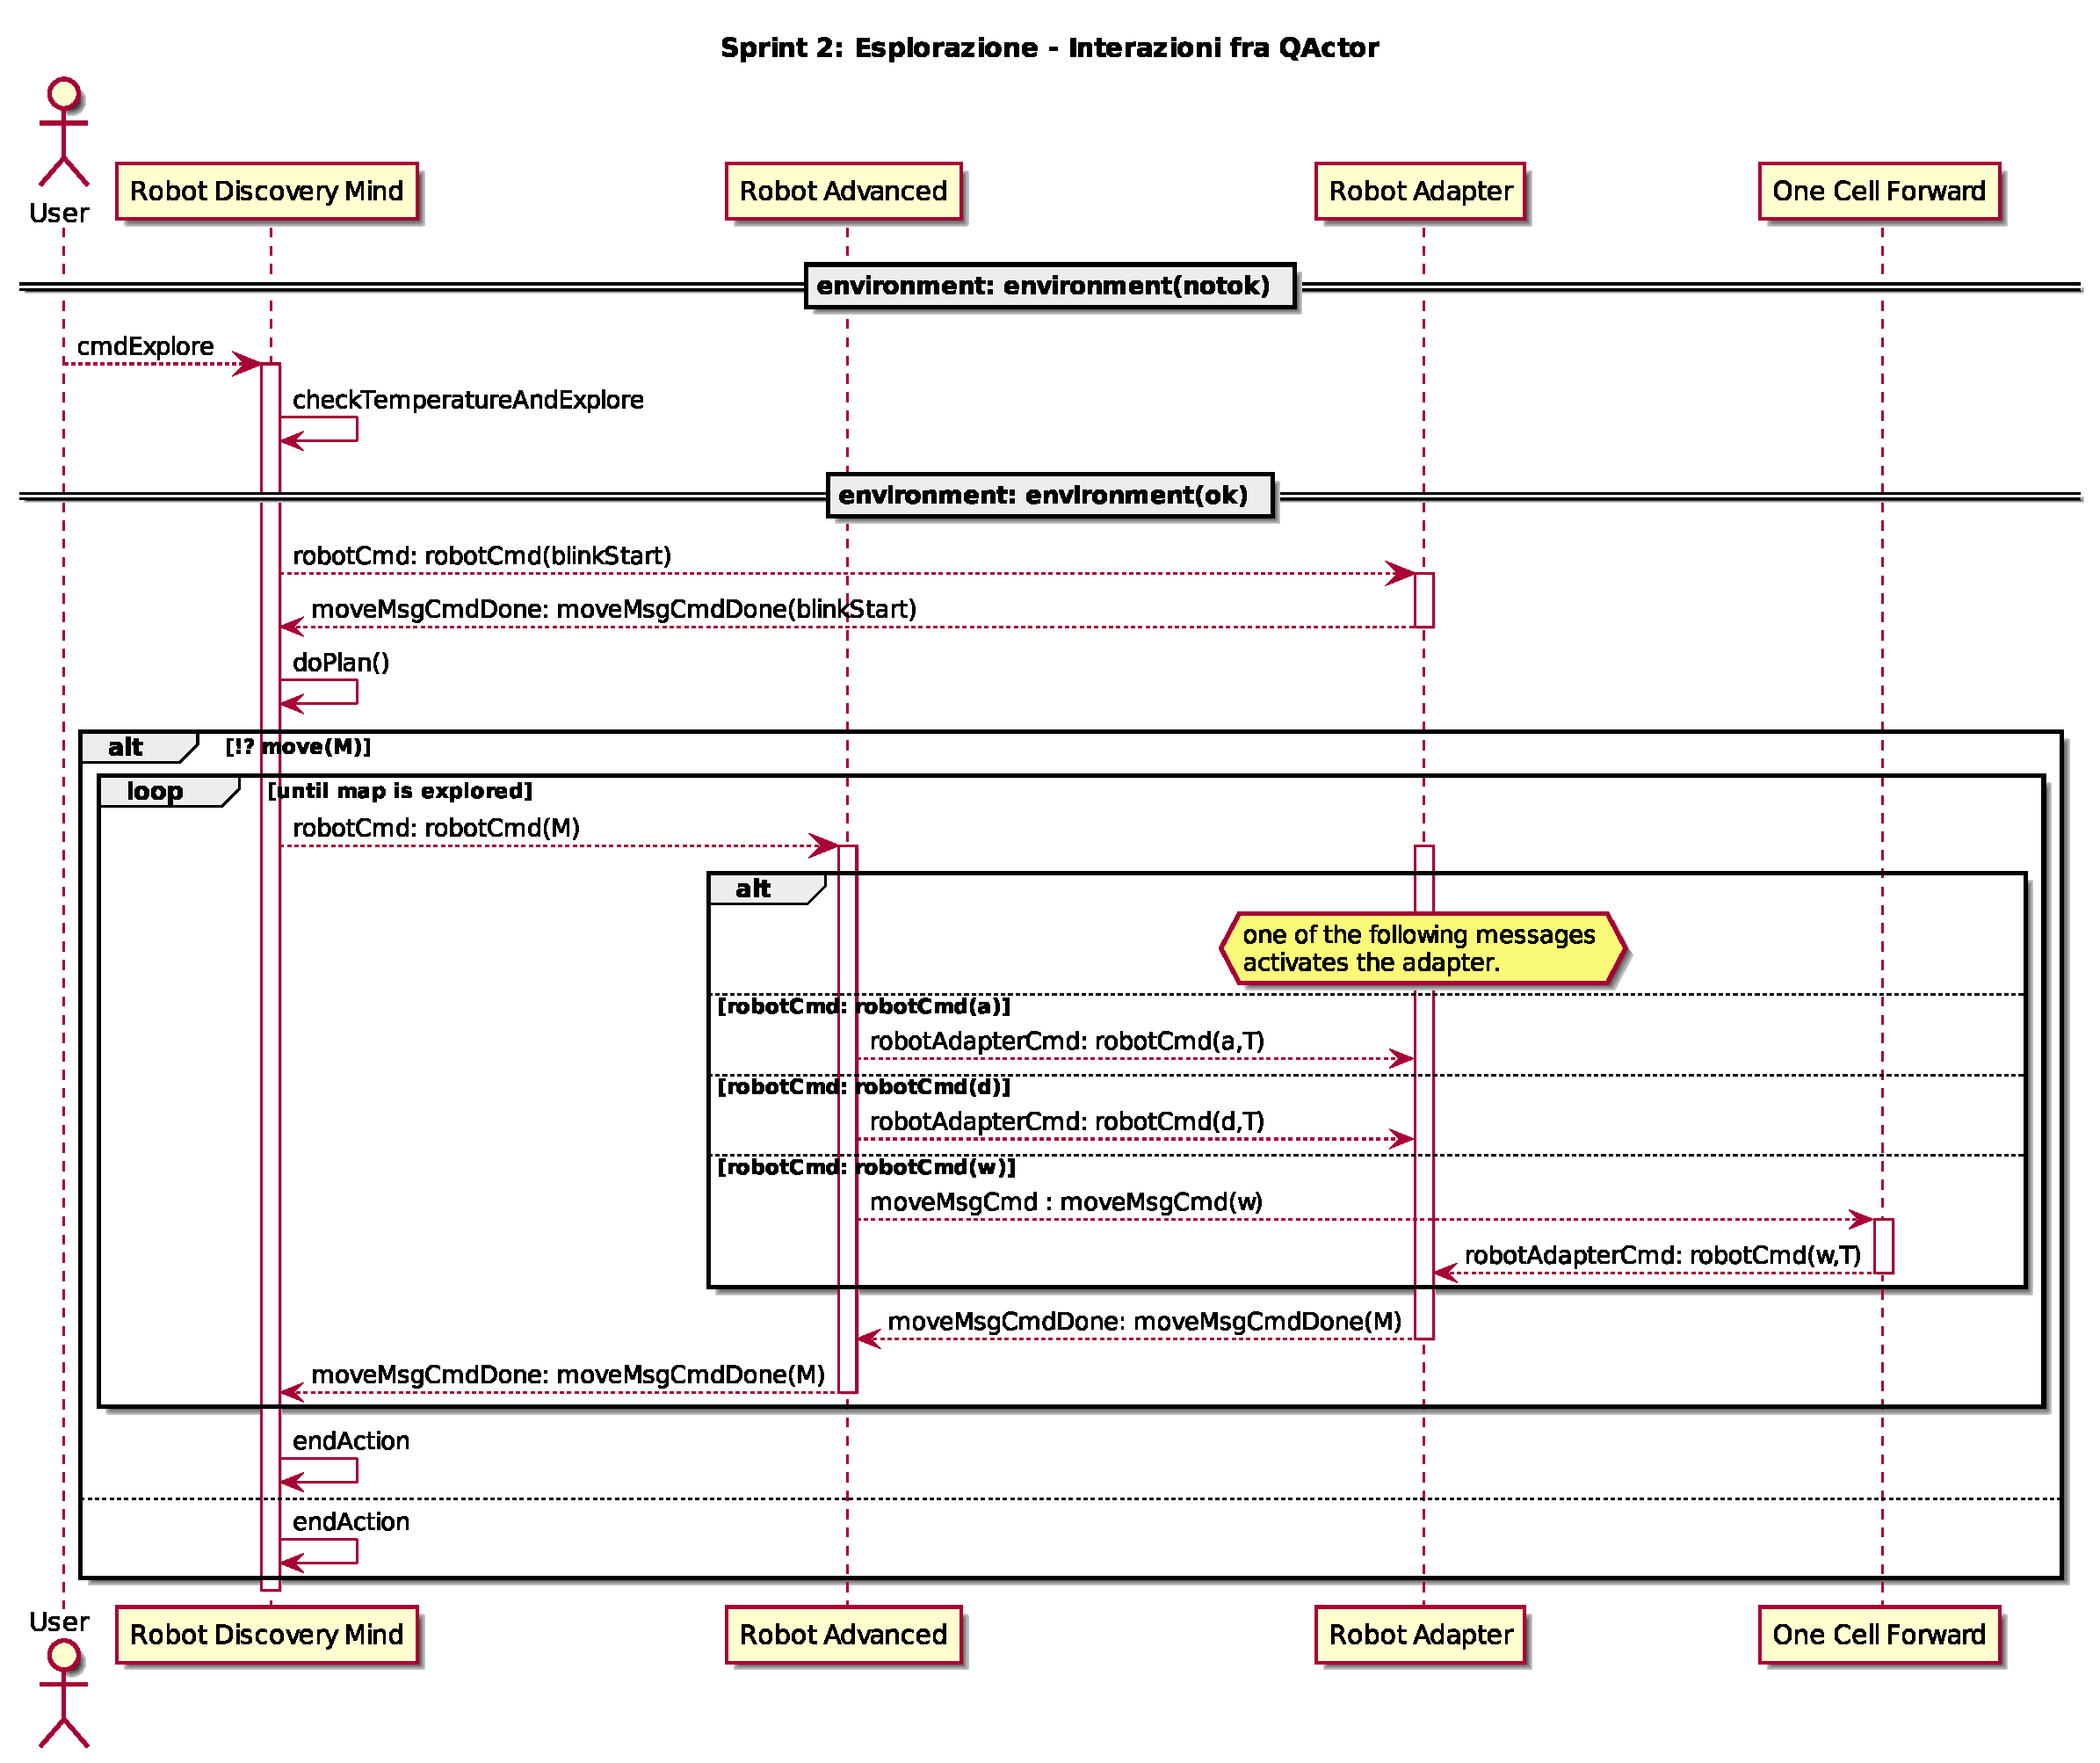
\includegraphics[width=\textwidth]{res/sprint2/explore}
  \caption{Schema UML che riassume le interazioni tra \texttt{QActor} per l'esplorazione}%
  \label{fig:sp2:explore}
\end{figure}

\newpage

\subsection[Rappresentazione formale]{Rappresentazione formale in output alla fase di analisi del problema}\labelssec{sp2:qa}

Data la dimensione del file di metamodello \texttt{robot.qa}, di seguito sono rappresentati in blocchi separati parti il codice di metamodello dei singoli attori maggiormente coinvolti:

% WORLD OBSERVER
% \lstinputlisting[%
%   firstline=61,%
%   lastline=80,%
%   language=qa%
% ]{res/sprint2/robot.qa}

% ROBOT ADAPTER
\lstinputlisting[%
  firstline=83,%
  lastline=116,%
  language=qa%
]{res/sprint2/robot.qa}

% ROBOT ADVANCED
\lstinputlisting[%
  firstline=118,%
  lastline=176,%
  language=qa%
]{res/sprint2/robot.qa}

% ONE CELL FORWARD
\lstinputlisting[%
  firstline=178,%
  lastline=228,%
  language=qa%
]{res/sprint2/robot.qa}

% DISCOVERY MIND
% \lstinputlisting[%
%   firstline=230,%
%   lastline=421,%
%   language=qa%
% ]{res/sprint2/robot.qa}

% RETRIEVER MIND
% \lstinputlisting[%
%   firstline=423,%
%   lastline=452,%
%   language=qa%
% ]{res/sprint2/robot.qa}

% CONSOLE
% \lstinputlisting[%
%   firstline=454,%
%   lastline=511,%
%   language=qa%
% ]{res/sprint2/robot.qa}

\subsection{Progettazione e Test planning}\labelssec{sp2:project}

In questa fase si è definito un piano di lavoro per la realizzazione concreta delle soluzioni individuate durante la fase di analisi:
in particolare, poiché il punto focale di questo sprint era l'esplorazione e il planning, si è realizzata l'integrazione delle soluzioni fornite dalla \textit{software house} all'interno del codice realizzato per questo progetto.

Non è stato ritenuto necessario definire \textit{unit test} per quanto importato dalla \textit{codebase} della \textit{software house}, in quanto è codice fornito come già testato;
per quanto riguarda il testing dell'integrazione, si è deciso di effettuare un testing empirico sfruttando il robot virtuale già citato in precedenza.

\subsection{Sprint Review}\labelssec{sp2:review}

Come per lo \nameref{sec:sprint1}, l'interazione con il committente è stata limitata a uno scambio di email, in quanto non erano presenti elementi interessanti da discutere.
